\documentclass{beamer}
\usepackage{amsmath}
\mode<presentation>
\usepackage{amssymb}
%\usepackage{advdate}
\usepackage{adjustbox}
\usepackage{subcaption}
\usepackage{enumitem}
\usepackage{multicol}
\usepackage{mathtools}
\usepackage{listings}
\usepackage{url}
\def\UrlBreaks{\do\/\do-}
\usetheme{Boadilla}
\usecolortheme{lily}
\setbeamertemplate{footline}
{
  \leavevmode%
  \hbox{%
  \begin{beamercolorbox}[wd=\paperwidth,ht=2.25ex,dp=1ex,right]{author in head/foot}%
    \insertframenumber{} / \inserttotalframenumber\hspace*{2ex} 
  \end{beamercolorbox}}%
  \vskip0pt%
}
\setbeamertemplate{navigation symbols}{}

\providecommand{\nCr}[2]{\,^{#1}C_{#2}} % nCr
\providecommand{\nPr}[2]{\,^{#1}P_{#2}} % nPr
\providecommand{\mbf}{\mathbf}
\providecommand{\pr}[1]{\ensuremath{\Pr\left(#1\right)}}
\providecommand{\qfunc}[1]{\ensuremath{Q\left(#1\right)}}
\providecommand{\sbrak}[1]{\ensuremath{{}\left[#1\right]}}
\providecommand{\lsbrak}[1]{\ensuremath{{}\left[#1\right.}}
\providecommand{\rsbrak}[1]{\ensuremath{{}\left.#1\right]}}
\providecommand{\brak}[1]{\ensuremath{\left(#1\right)}}
\providecommand{\lbrak}[1]{\ensuremath{\left(#1\right.}}
\providecommand{\rbrak}[1]{\ensuremath{\left.#1\right)}}
\providecommand{\cbrak}[1]{\ensuremath{\left\{#1\right\}}}
\providecommand{\lcbrak}[1]{\ensuremath{\left\{#1\right.}}
\providecommand{\rcbrak}[1]{\ensuremath{\left.#1\right\}}}
\theoremstyle{remark}
\newtheorem{rem}{Remark}
\newcommand{\sgn}{\mathop{\mathrm{sgn}}}
\providecommand{\abs}[1]{\left\vert#1\right\vert}
\providecommand{\res}[1]{\Res\displaylimits_{#1}} 
\providecommand{\norm}[1]{\lVert#1\rVert}
\providecommand{\mtx}[1]{\mathbf{#1}}
\providecommand{\mean}[1]{E\left[ #1 \right]}
\providecommand{\fourier}{\overset{\mathcal{F}}{ \rightleftharpoons}}
%\providecommand{\hilbert}{\overset{\mathcal{H}}{ \rightleftharpoons}}
\providecommand{\system}{\overset{\mathcal{H}}{ \longleftrightarrow}}
	%\newcommand{\solution}[2]{\textbf{Solution:}{#1}}
%\newcommand{\solution}{\noindent \textbf{Solution: }}
\providecommand{\dec}[2]{\ensuremath{\overset{#1}{\underset{#2}{\gtrless}}}}
\newcommand{\myvec}[1]{\ensuremath{\begin{pmatrix}#1\end{pmatrix}}}
\newcommand{\mydet}[1]{\ensuremath{\begin{vmatrix}#1\end{vmatrix}}}
\let\vec\mathbf

\lstset{
%language=C,
frame=single, 
breaklines=true,
columns=fullflexible
}

\numberwithin{equation}{section}

\title{2.10.85}
\author{Rushil Shanmukha Srinivas \\EE25BTECH11057 \\ Electrical Enggineering ,\\IIT Hyderabad.}

\date{\today} 
\begin{document} 

\begin{frame}
\titlepage
\end{frame}

\section*{Outline}
\begin{frame}
\tableofcontents
\end{frame}
\section{Problem}
\begin{frame}
\frametitle{Problem Statement}
\textbf{Question} : Let P be the plane 3x+2y+3z=16 and let S: $\alpha\hat{i} + \beta\hat{j} + \gamma\hat{k} $ ,where $\alpha+\beta+\gamma=7$ and the distance of $(\alpha,\beta,\gamma)$ from the plane is $2/{\sqrt{22}}$ .Let $\vec{u},\vec{v},\vec{w}$ be three distinct vectors in S such that $|\vec{u}-\vec{v}|=|\vec{v}-\vec{w}|=|\vec{w}-\vec{u}|$. Let V be the volume of the parallelopiped determined by vectors $\vec{u},\vec{v},\vec{w}$. Then the value of (80/3)V is 

\end{frame}
\section{Solution}
\subsection{Distance between point and plane,Line Equation}
\begin{frame}
\frametitle{Distance between point and plane,Line Equation}
%\framesubtitle{Literature}
\textbf{Solution} :
\begin{align}
P:\; \vec{n}^\top \vec{x} = c,\qquad \vec{n}=\myvec {3\\2\\3}\;c=16.
\end{align}

The distance of point $\vec{P_0}=\myvec{\alpha\\ \beta\\ \gamma}$ from the plane is
\begin{align}
\operatorname{dist}(\vec{P_0},P)=\frac{|\vec{n}^\top \vec{P_0} - c|}{\norm{\vec{n}}}
\end{align}
Given $\alpha+\beta+\gamma=7$ and $\operatorname{dist}(\vec{P_0},P)=\tfrac{2}{\sqrt{22}}$, we have
\begin{align}
\frac{|3\alpha+2\beta+3\gamma-16|}{\sqrt{22}}=\frac{2}{\sqrt{22}}
\;\;\Longrightarrow\;\; \vec{n}^\top \vec{P_0}=18 \;\;\text{or}\;\; \vec{n}^\top \vec{P_0}=14.
\end{align}

Thus $S$ lies on the intersections
\end{frame}
\begin{frame}
\begin{align}
\Pi:\; \vec{m}^\top \vec{x}=7,\qquad \vec{m}=\myvec{1\\1\\1},
\end{align}
with
\begin{align}
P_+: \vec{n}^\top \vec{x}=18,\qquad P_-:\vec{n}^\top \vec{x}=14.
\end{align}
textbf{(i) Intersection of $\vec{m}^\top \vec{x}=7$ and $\vec{n}^\top \vec{x}=18$.}\\
Write the augmented system in matrix form:
\begin{align}
\myvec
{1 & 1 & 1 &\vrule& 7\\[4pt]
3 & 2 & 3 &\vrule& 18} \xrightarrow{R_2 \longrightarrow R_2-3R_1}
\myvec{
1 & 1 & 1 &\vrule& 7\\[4pt]
0 & -1 & 0 &\vrule& -3}.
\end{align}
From the second row we get  $y=3$. Substitute into $x+y+z=7$:
\begin{align}
x+3+z=7 \quad\Longrightarrow\quad z=4-x.
\end{align}
So the line is
\begin{align}
\vec{L_1} = \myvec{0\\3\\4} + k_1\myvec{1\\0\\-1} = \vec{a} + k_1 \vec{d} 
\end{align}
\end{frame}
\begin{frame}
\textbf{(ii) Intersection of $\vec{m}^\top \vec{x}=7$ and $\vec{n}^\top \vec{x}=14$.}\\
The augmented matrix is
\begin{align}
\myvec
{1 & 1 & 1 &\vrule& 7\\[4pt]
3 & 2 & 3 &\vrule& 14} \xrightarrow{R_2 \longrightarrow R_2-3R_1}
\myvec
{1 & 1 & 1 &\vrule& 7\\[4pt]
0 & -1 & 0 &\vrule& -7}.
\end{align}
So  $y=7$. From $x+y+z=7$ we get
\begin{align}
x+7+z=7 \quad\Longrightarrow\quad z=-x.
\end{align}
\begin{align}
\vec{L_2} = \myvec{0\\7\\0} + k_2\myvec{1\\0\\-1} = \vec{b} + k_2 \vec{d}
\end{align}
 hence the two lines are parallel.
 

\end{frame}
\subsection{Least Squares Solution }
\begin{frame}
\frametitle{Least Squares Solution}

 \textbf{(iii) Perpendicular distance between the two parallel lines}:
 $\vec{P}=\vec{a}+p_1 \vec{d} \ and\ \vec{Q}=\vec{b}+p_2 \vec{d} \ be \ 2 points\ on\ \vec{L_1},\vec{L_2}. $
\begin{align} 
perpendicular\ distance = \operatorname{dist}(\vec{P},\vec{Q}) ,\vec{M}=\myvec{\vec{d} & \vec{d}} 
\end{align}
 \begin{align}
 \vec{M}^\top(a-b) + \vec{M}^\top\vec{M}\myvec{p_1\\-p_2} = 0 , 
 \end{align}
 \begin{align}
 \myvec{\vec{d}\\\vec{d}}(a-b) + \myvec{\vec{d}\\\vec{d}}\myvec{\vec{d}&\vec{d}}\myvec{p_1\\-p_2} = 0
 \end{align}
On solving we get , 
\begin{align}
p_1 - p_2 = 2 \ take \ p_1=2 \ and \ p_2=0
\end{align}
 Points are $\vec{P}=\myvec{2\\3\\2} , \vec{Q}=\myvec{0\\7\\0},\vec{P}-\vec{Q}=\myvec{2\\-4\\2}$
 \begin{align}
Distance = D= {\norm{\vec{P}-\vec{Q}}} = \sqrt{24} 
\end{align}
\end{frame}

\subsection{Area and Volume}
\begin{frame}
\frametitle{Area and Volume}
\textbf{(iv) Area of the equilateral triangle formed by $\vec{u},\vec{v},\vec{w}$}:
As the two lines are parallel and let s = length of side of triangle
\begin{align}
D = \frac{\sqrt{3}s}{2} \Longrightarrow s = 4\sqrt{2}
\end{align}
\begin{align}
\text Area \ of\ the\ equilateral\ triangle = A = \frac{\sqrt{3}s^2}{4} = 8\sqrt{3} 
\end{align}
\textbf{(v) Volume of the parallelepiped determined by three vectors $\vec{u},\vec{v},\vec{w}$}:
$Volume\ of\ Parallelepiped = 6(Volume\ of\ Tetrahedron) = 2\times base\ area\times height$
\begin{align}
height=h=\frac{|\vec{m}^\top\vec{O}-c|}{\norm{\vec{m}}}=\frac{|0-7|}{\sqrt{3}}=\frac{7}{\sqrt{3}}
\end{align}
\begin{align}
Volume = 2\times8\sqrt{3}\times\frac{7}{\sqrt{3}} = 112
\end{align}
\begin{align}
\frac{80}{3}V = \frac{80}{3}\times 112 = \frac{8960}{3}.
\end{align}
\end{frame}
\subsection{Plots}
\begin{frame}
\frametitle{Plots}
\begin{figure}
\centering
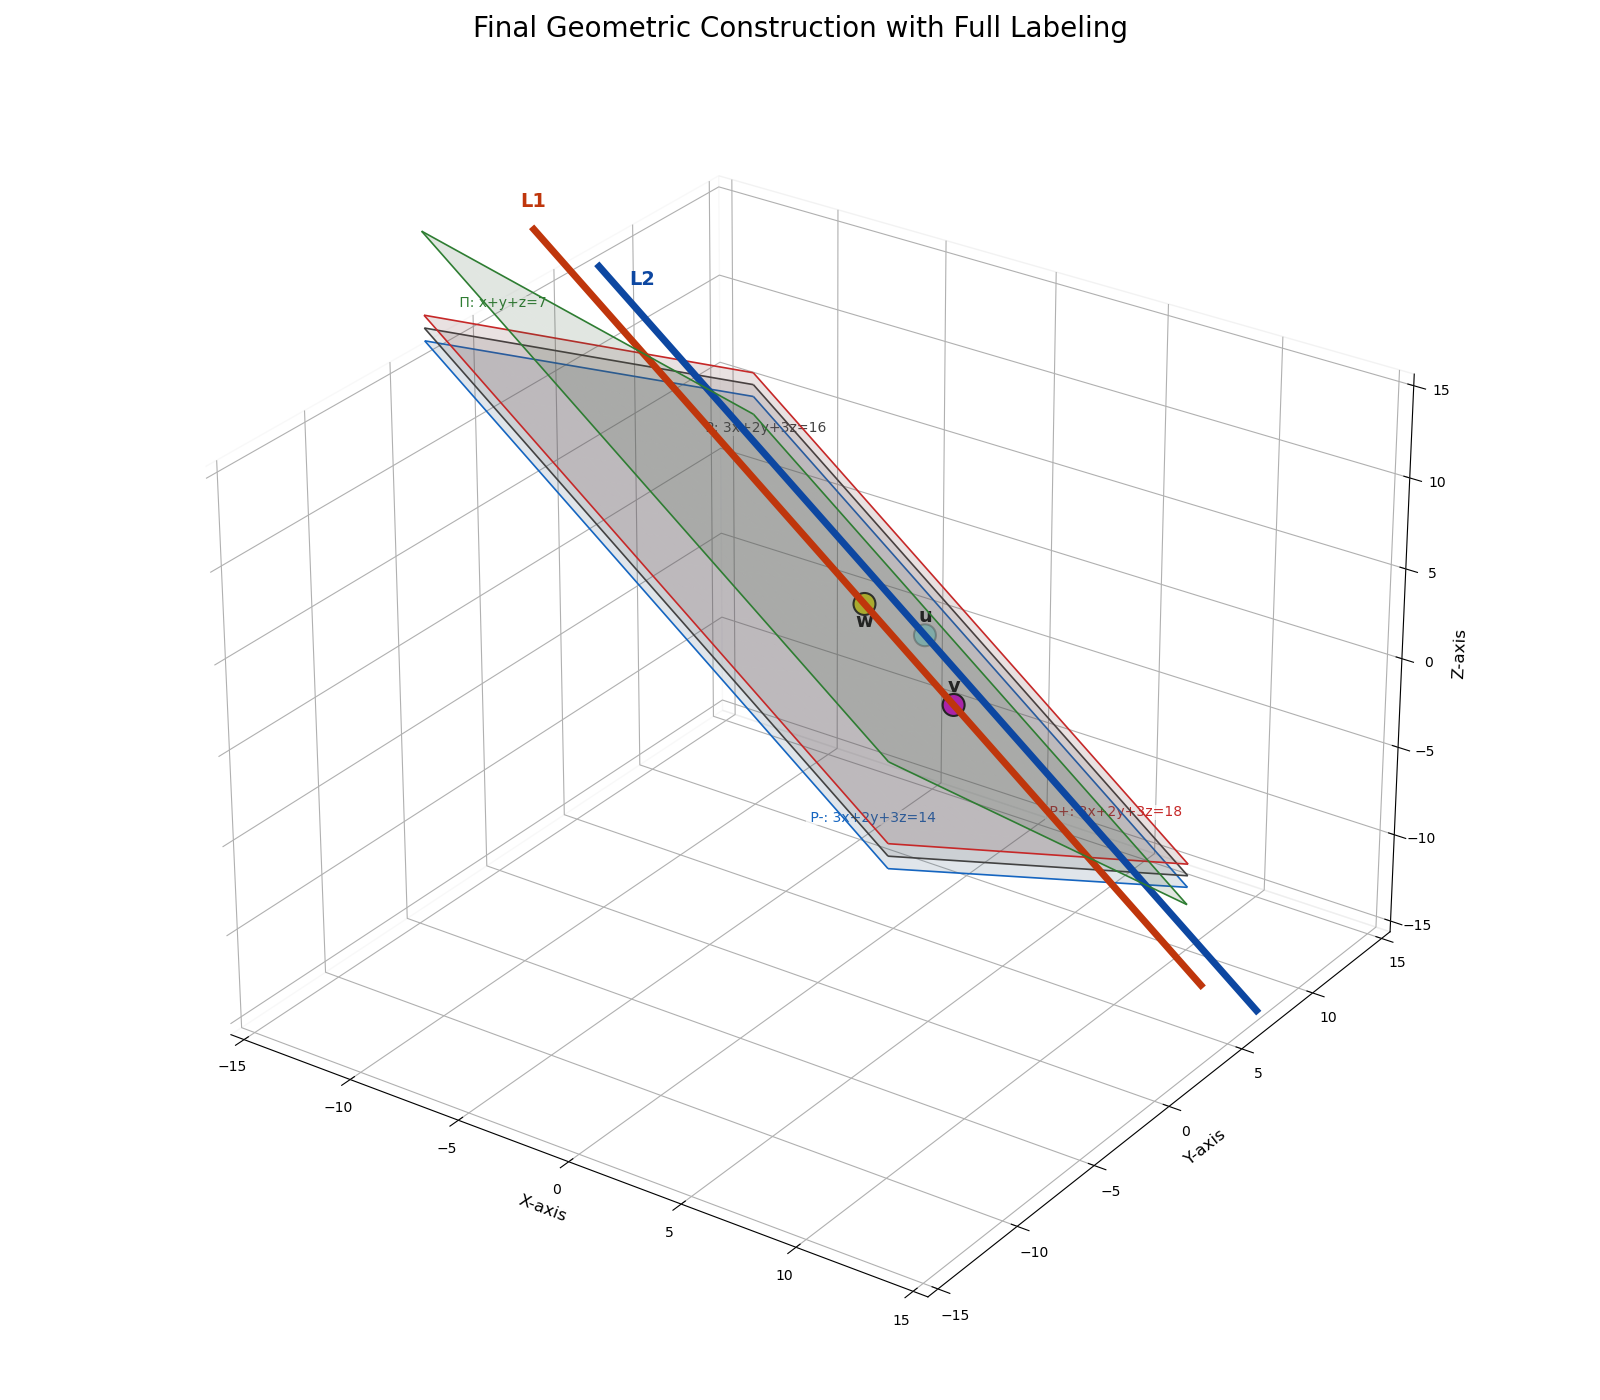
\includegraphics[width=0.8\columnwidth]{figs/fig5_.png}
\caption{fig : Representation of Planes and vectors}
\label{Fig5}
\end{figure}
\end{frame}
\section{C Code}
\begin{frame}[fragile]
\frametitle{C Code }
\begin{lstlisting}[language=C]
#include <stdio.h>
#include <math.h>

// Function to compute determinant of 3x3 matrix
double determinant(double a[3][3]) {
    return a[0][0]*(a[1][1]*a[2][2] - a[1][2]*a[2][1])
         - a[0][1]*(a[1][0]*a[2][2] - a[1][2]*a[2][0])
         + a[0][2]*(a[1][0]*a[2][1] - a[1][1]*a[2][0]);}
int main() {
    // Two planes:
    // Plane P: 3x+2y+3z=16
    // Plane S: x+y+z=7
    // Solve intersection line between P and S
    // Choose basis for S: let
    // a = (1,-1,0), b = (1,0,-1) → both satisfy x+y+z=0
    \end{lstlisting}
    \end{frame}
    \begin{frame}[fragile]
    \begin{lstlisting}
    // So general point on S: (7,0,0) + s*a + t*b
    // Constraint from P: 3x+2y+3z = 14 or 18 (distance condition)
    
    // Pick "14" first.
    // Solve quickly: Intersection point
    double u[3] = {2,3,2};
    double v[3] = {-2,3,6};
    double w[3] = {-2,7,2};
    
    // Put in matrix
    double M[3][3] = {
        {u[0], v[0], w[0]},
        {u[1], v[1], w[1]},
        {u[2], v[2], w[2]}};
    // Determinant
    double det = determinant(M);
    double V = fabs(det);
    double result = (80.0/3.0) * V;
\end{lstlisting}
\end{frame}
\begin{frame}[fragile]
\begin{lstlisting}
    printf("Chosen vectors:\n");
    printf("u = (%.2lf, %.2lf, %.2lf)\n", u[0], u[1], u[2]);
    printf("v = (%.2lf, %.2lf, %.2lf)\n", v[0], v[1], v[2]);
    printf("w = (%.2lf, %.2lf, %.2lf)\n", w[0], w[1], w[2]);
    printf("Determinant = %.2lf\n", det);
    printf("Volume V = %.2lf\n", V);
    printf("Final (80/3)*V = %.2lf\n", result);

    return 0;
}

\end{lstlisting}
\end{frame}

\section{Python Code}
\begin{frame}[fragile]
\frametitle{Python : call\_c.py}
\begin{lstlisting}
import ctypes
import os

# Load shared library
lib = ctypes.CDLL(os.path.abspath("./libvolume.so"))

# Set return types
lib.get_determinant.restype = ctypes.c_double
lib.get_volume.restype = ctypes.c_double
lib.compute_volume.restype = ctypes.c_double
lib.get_u.restype = ctypes.c_double
lib.get_v.restype = ctypes.c_double
lib.get_w.restype = ctypes.c_double

# Fetch vectors u, v, w
u = [lib.get_u(i) for i in range(3)]
v = [lib.get_v(i) for i in range(3)]
\end{lstlisting}
\end{frame}
\begin{frame}[fragile]
\begin{lstlisting}
w = [lib.get_w(i) for i in range(3)]

# Fetch determinant, volume, and final result
det = lib.get_determinant()
V = lib.get_volume()
result = lib.compute_volume()

# Print everything
print("Vector u =", u)
print("Vector v =", v)
print("Vector w =", w)
print("Determinant =", det)
print("Volume V =", V)
print("Final (80/3)*V =", result)

\end{lstlisting}
\end{frame}

\begin{frame}[fragile]
\frametitle{Python Code for Plotting}
\begin{lstlisting}[language=Python] 

import numpy as np
import matplotlib.pyplot as plt
from mpl_toolkits.mplot3d import art3d

# --- Create the Figure ---
fig = plt.figure(figsize=(16, 14))
ax = fig.add_subplot(111, projection='3d')

# --- Generate Grid and Define Boundaries ---
lim = 10
x_range = np.linspace(-lim, lim, 50)
y_range = np.linspace(-lim, lim, 50)
X, Y = np.meshgrid(x_range, y_range)

# --- AESTHETIC AND COLOR DEFINITIONS ---
# Define surface colors and darker corresponding outline colors
\end{lstlisting}
\end{frame}
\begin{frame}[fragile]
\begin{lstlisting}
colors = {
    'P+':  {'surface': '#E57373', 'outline': '#C62828'}, # Light Red / Dark Red
    'P-':  {'surface': '#64B5F6', 'outline': '#1565C0'}, # Light Blue / Dark Blue
    'Π':   {'surface': '#81C784', 'outline': '#2E7D32'}, # Light Green / Dark Green
    'P':   {'surface': '#BDBDBD', 'outline': '#424242'}  # Light Grey / Dark Grey}
# --- PLOTTING PLANES WITH SURFACES AND OUTLINES ---
# Function to plot a plane with its surface and a dark outline
def plot_complete_plane(Z, color_pair):
    # Plot the highly transparent surface
    ax.plot_surface(X, Y, Z, alpha=0.15, color=color_pair['surface'], rstride=5, cstride=5, edgecolor='none')
    # Plot a crisp, dark wireframe outline
    ax.plot_wireframe(X, Y, Z, color=color_pair['outline'], linewidth=1.2, rstride=100, cstride=100)
\end{lstlisting}
\end{frame}
\begin{frame}[fragile]
\begin{lstlisting}
# 1. Plane Π: x + y + z = 7
Z_Pi = 7 - X - Y
plot_complete_plane(Z_Pi, colors['Π'])
# 2. Plane P+: 3x+2y+3z=18
Z_P_plus = (18 - 3*X - 2*Y) / 3
plot_complete_plane(Z_P_plus, colors['P+'])
# 3. Plane P-: 3x+2y+3z=14
Z_P_minus = (14 - 3*X - 2*Y) / 3
plot_complete_plane(Z_P_minus, colors['P-'])
# 4. Original Plane P: 3x+2y+3z=16
Z_P = (16 - 3*X - 2*Y) / 3
plot_complete_plane(Z_P, colors['P'])

# --- EMPHASIZE AND LABEL LINES/POINTS ---
FOREGROUND_ZORDER = 10
t_start, t_end = -15, 15
t_lines = np.linspace(t_start, t_end, 100)
d = np.array([1, 0, -1])  # Direction vector
\end{lstlisting}
\end{frame}
\begin{frame}[fragile]
\begin{lstlisting}
# Line L1
a = np.array([0, 3, 4])
L1 = a + t_lines[:, np.newaxis] * d
ax.plot(L1[:, 0], L1[:, 1], L1[:, 2], color='#BF360C', lw=5, zorder=FOREGROUND_ZORDER) # Deep Orange
# Line L2
b = np.array([0, 7, 0])
L2 = b + t_lines[:, np.newaxis] * d
ax.plot(L2[:, 0], L2[:, 1], L2[:, 2], color='#0D47A1', lw=5, zorder=FOREGROUND_ZORDER) # Deep Blue
# Points u, v, w
point_size = 250
u, s = b, 4 * np.sqrt(2)
t_proj = np.dot(u - a, d) / np.dot(d, d)
M = a + t_proj * d
dist_M_v = s/2
v = M + (dist_M_v / np.linalg.norm(d)) * d
w = M - (dist_M_v / np.linalg.norm(d)) * d
\end{lstlisting}
\end{frame}
\begin{frame}[fragile]
\begin{lstlisting}
ax.scatter([u[0],v[0],w[0]], [u[1],v[1],w[1]], [u[2],v[2],w[2]],
           color=['cyan','magenta','yellow'], s=point_size, ec='black', lw=1.5, zorder=FOREGROUND_ZORDER + 1)

# --- ADDING ALL LABELS (PLANES, LINES, AND POINTS) ---
# Plane Labels
plane_label_props = {'ha':'center', 'va':'center', 'fontsize':10, 'bbox':dict(facecolor='white', alpha=0.7, ec='none', pad=0.2)}
ax.text(-8,-8, 7-(-8)-(-8), " Π: x+y+z=7 ", color=colors['Π']['outline'], **plane_label_props)
ax.text(8, 8, (18-3*8-2*8)/3, " P+: 3x+2y+3z=18 ", color=colors['P+']['outline'], **plane_label_props)
ax.text(8,-8, (14-3*8-2*(-8))/3, " P-: 3x+2y+3z=14 ", color=colors['P-']['outline'], **plane_label_props)
ax.text(-8, 8, (16-3*(-8)-2*8)/3, " P: 3x+2y+3z=16 ", color=colors['P']['outline'], **plane_label_props)
# Line Endpoint Labels
line_label_props = {'ha':'center', 'va':'center', 'fontsize':14, 'fontweight':'bold'}
\end{lstlisting}
\end{frame}
\begin{frame}[fragile]
\begin{lstlisting}
l1_start_pos = a + t_start * d
l2_start_pos = b + t_start * d
ax.text(l1_start_pos[0], l1_start_pos[1], l1_start_pos[2] + 1.5, "L1", color='#BF360C', **line_label_props)
ax.text(l2_start_pos[0] + 2, l2_start_pos[1], l2_start_pos[2] , "L2", color='#0D47A1', **line_label_props)
# Point Labels (u, v, w)
point_label_props = {'ha':'center', 'va':'bottom', 'fontsize':14, 'fontweight':'bold'}
ax.text(u[0], u[1], u[2] + 0.5, 'u', color='black', **point_label_props)
ax.text(v[0], v[1], v[2] + 0.5, 'v', color='black', **point_label_props)
ax.text(w[0], w[1], w[2] - 1.5, 'w', color='black', **point_label_props) # slight offset for w

# --- FINAL PLOT SETUP ---
ax.view_init(elev=28, azim=-55)
\end{lstlisting}
\end{frame}
\begin{frame}[fragile]
\begin{lstlisting}
ax.set_xlim(-15, 15); ax.set_ylim(-15, 15); ax.set_zlim(-15, 15)
ax.set_xlabel('X-axis', fontsize=12); ax.set_ylabel('Y-axis', fontsize=12); ax.set_zlabel('Z-axis', fontsize=12)
ax.set_title('Final Geometric Construction with Full Labeling', fontsize=20, pad=20)

# Clean background
ax.xaxis.pane.fill=False; ax.yaxis.pane.fill=False; ax.zaxis.pane.fill=False
ax.grid(True, linestyle=':', alpha=0.5)

plt.tight_layout()
plt.savefig("../figs/fig5_.png")
plt.show()
\end{lstlisting}
\end{frame}


\end{document}
  